In this paper we are interested in the stationary 
Fokker-Planck equation
\begin{equation}
\begin{aligned}
&\mathcal L p \stackrel{\rm def}{=}
  -\nabla \cdot(\mu p) + D\odot\nabla^2p=0,\qquad\mathbf x\in\mathbb R^d\\
  &\int_{\mathbb R^d}p(\mathbf x)\,d\mathbf x = 1\label{eq:SFPE-0}
\end{aligned}
\end{equation}
Here $\odot$ is the Hadamard product, $\nabla^2$ denotes Hessian, $D=\frac{1}{2}\sigma\sigma^\top$,  $\mu\in C^1(\mathbb R^d; \mathbb R^d)$ is a non-solenoidal vector field i.e. $\nabla\cdot\mu\not\equiv0$ in $\mathbb R^d$ and $\sigma\in C(\mathbb R^d; \mathbb R^{d\times l})$  matrix-valued function such that $D$ is positive-definite.
The operator $\mathcal L$ is known as the \textit{Fokker-Planck operator} (FPO). The goal of this work is to devise an algorithm to find a non-trivial zero of  $\mathcal L$ in a mesh-free manner that works well in dimensions that are challenging for classical PDE-solvers. Note that when $\mu$ is solenoidal The motivations behind choosing to find a non-trivial zero of $\mathcal L$ rather than solving \eqref{eq:SFPE-0} are as follows. 
\begin{itemize}
    \item Numerical integration suffers from the curse of dimensionality \cite{hinrichs2014curse} and consequently the normalization constraint is extremely challenging to implement in high dimensions.
    \item The end goal is to devise an algorithm to solve time-dependent FPEs with unique solutions which we describe in the sequel. It turns out, knowing a non-trivial zero of $\mathcal L$, even if unnormalized, is enough to find the normalized solution to the time-dependent FPE.
    \item When $\mu$ is solenoidal every constant function is a zero of $\mathcal L$. In this special case if the corresponding time-dependent FPE has a unique solution, we would not require a non-trivial zero of $\mathcal L$ to calculate it, as we will see in the sequel.
    \item Lastly, rather than trying to force normalization during the computation of a non-trivial zero, it is much more economical to integrate the zero at the end to find the normalization constant at a one-time cost. Quasi Monte Carlo \cite{leobacher2014introduction} or deep learning methods like i-flow \cite{gao2020flow} can be used for this purpose. 
\end{itemize}
 

Although our method is perfectly valid for any matrix-valued $\sigma$ that gives rise to a positive definite $D$, in the demonstrations we use the form  $\sigma = c I_d$ where $c$ is a positive constant and $I_d$ is the $d\times d$ identity matrix. This allows us to abuse notation and use $\sigma$ and $D$ as scalar quantities. With this simplification our equation becomes, 
\begin{align}
    \mathcal L p= -\nabla\cdot(\mu p) + D\Delta p=0\label{eq:SFPE-1}
\end{align}
where $\Delta$ is the Laplacian operator. 

Since we approximate a solution to \eqref{eq:SFPE-1} with a neural network, it is sensible to consider strong solutions. We therefore  restrict our search space of functions to $W^{1, 2}(\mathbb R^d)\cap C^2(\mathbb R^d)$ with the norm,
\begin{align}
\|\phi\|_{1, 2} =\left(\int_{\mathbb R^d}|\phi|^2\right)^{\frac{1}{2}} + \left(\int_{\mathbb R^d}\|\nabla\phi\|_2^2\right)^{\frac{1}{2}}\label{eq:def-Sobolev-norm}
\end{align}
Sobolev spaces are frequently encountered while studying elliptic PDEs and therefore are very well-studied \cite{brezis2011functional},\cite{kilpelainen1994weighted}.  This choice of function space enables us to prove uniqueness of solutions to the SFPEs that we will encounter in this paper, see appendix~\ref{ssec-unique} for details. Moreover, density of arbitrary-size neural networks in the space of continuous functions \cite{pinkus1999approximation} and non-closedness of fixed-size neural networks in Sobolev spaces \cite{mahan2021nonclosedness} are good justifications for our algorithm, see section~\ref{ssec-infinite-to-finite}.

\section{Examples}\label{sec-examples}
From an algorithmist's perspective it is important to have access to a class of equations on which our algorithm can be validated easily. Since classical methods do not work satisfactorily for our problem dimensions, the only other way is to use those equations, for which the analytical solutions are known, as the validating examples.  
\subsection{Gradient systems}
To that end a very convenient class of equations is where the drift $\mu$ can be written as the gradient of a potential function $V$,

\begin{align}
    \mu = -\nabla V\label{eq:mu-grad}
\end{align}
To see why this structure of $\mu$ leads to analytical solutions of SFPEs, note that if $p=e^f$ is a solution to the SFPE then according to \eqref{eq:SFPE-1} we have 
\begin{align}
    &\mathcal -\nabla\cdot(e^f\mu) + D\Delta e^f =0\\
    \implies&  -\nabla\cdot \mu - \mu \cdot \nabla f + D\left(\|\nabla f\|_2^2 + \Delta f\right) =0 \label{eq:log-transform-0}\\
    \implies&(\nabla + \nabla f)\cdot(D\nabla f -\mu) =0\label{eq:log-factor}\\
    \implies&(\nabla + \nabla f)\cdot(\nabla (Df + V)) =0\label{eq:log-factor-V}    
\end{align}
so we can find one solution by simply setting the second term in the RHS of \eqref{eq:log-factor-V} to be zero which gives us
\begin{align}
    &\nabla(Df + V) = \mathbf 0\\
    \implies& f =\ln c-\frac{V}{D}\\
    \implies& p= c\exp\left(-\frac{V}{D}\right)\label{eq:grad-sol}
\end{align}
where $c$ is the normalizing constant. So a solution in this special case is already known up to the normalizing constant. We refer to a system satisfying \eqref{eq:mu-grad} as a \textit{gradient system}.
In this paper we use the following gradient systems to validate our algorithm in high dimensions. 

\subsubsection{2D ring system}
For $d=2$, $V=(x^2+y^2-1)^2$ and $\mu=-\nabla V$ we get the following SFPE,
\begin{align}
     4(x^2+y^2-1)\left(x\frac{\partial p}{\partial x}+y\frac{\partial p}{\partial y}\right) + 8(2x^2+2y^2-1)p + D\Delta p=0 \label{eq:ring2D}
\end{align}
This system possesses a unique solution concentrated on around the unit circle. The proof of uniqueness using the method of Lyapunov functions is given in the appendix~\ref{sssec-2D-unique}. The corresponding ODE system has the unit circle as a global attractor. This is a recurring theme in all of our example problems. Such systems with attractors are of great interest in the study of dynamical systems \cite{ott1981strange} as well as filtering theory \cite{kontorovich2009non}. We solve this system for $D=1$.

\subsubsection{2nD ring system} We can daisy-chain the previous system to build decoupled systems in higher dimensions. In this case the potential is given by
\begin{align}
    V(\mathbf x)=\sum_{i=0}^{\frac{d}{2}-1}(x_{2i}^2+x_{2i+1}^2-1)^2,\qquad d=2n
\end{align}
Since our algorithm does not differentiate between coupled and decoupled systems, this example serves as a great high-dimensional test case. In a sequel we show how to solve the time-dependent FPEs which is intimately related to the method presented here and being decoupled, this system presents a great way to verify the time-dependent algorithm. This is important since analytical solutions for time-dependent FPEs are not known in general even for gradient systems. Uniqueness of solution for the 2nD ring system directly follows from the uniqueness of solution for the 2D ring system, again thanks to its decoupled nature. Here we solve this system for $n=1,2,3,4,5$ and $D=1$.
\subsection{Non-gradient Systems}
Not all $\mu$'s can however be represented as the gradient of a potential. We call the systems belonging to this complementary class, \textit{non-gradient systems}. Analytic solutions for these systems are not known in general.
\subsubsection{Noisy Lorenz-63 system}
One such example is the famous Lorenz-63 system, first proposed by Edward Lorenz \cite{lorenz1963deterministic} as an oversimplified model for atmospheric convection. This system and its variants like Lorenz-96 have since become staple test problems in the field of data assimilation \cite{carrassi2022data}, \cite{yeong2020particle}. We use the standard parameters to define the drift and solve the system for $D=50$. This exact system also appears as a test case in \cite{chen2018efficient}. The famous butterfly attractor associated with the corresponding ODE is shown in figure~\ref{fig:attractors}. This problem has a unique solution, for a proof see appendix~\ref{sssec-L63-unique}.
\begin{align}
    &\mu=[\alpha (y-x),\, x(\rho-z) - y,\, xy - \beta z]^\top\label{eq:mu-L63}\\
    &\alpha = 10 \,, \, \beta = \frac{8}{3}\,, \, \rho=28 \
\end{align}

\subsubsection{Noisy Thomas system}
Another example of a non-gradient system that we study is one for which the deterministic version was proposed by René Thomas~\cite{thomas1999deterministic}. It is a 3-dimensional system with cyclical symmetry in $x, y, z$ and the corresponding ODE system has a strange attractor which is depicted in figure~\ref{fig:attractors}.
We solve this system for $D=1$. This problem also has a unique solution, for a proof see appendix~\ref{sssec-Thomas-unique}.
\begin{align}
    &\mu=[\sin y - bx,\, \sin z - by,\, \sin x - by ]^\top\label{eq:mu-Thomas}\\
    &b =  0.2 
\end{align}

Since analytic solutions for non-gradient systems are not known, we stick to $d=3$ in this case. This is a dimension that can be reliably tackled with Monte Carlo simulations for comparison at a low computation cost. See \ref{ssec-MC-algo} for a description of the Monte Carlo algorithm.

\begin{figure}[!ht]
    \centering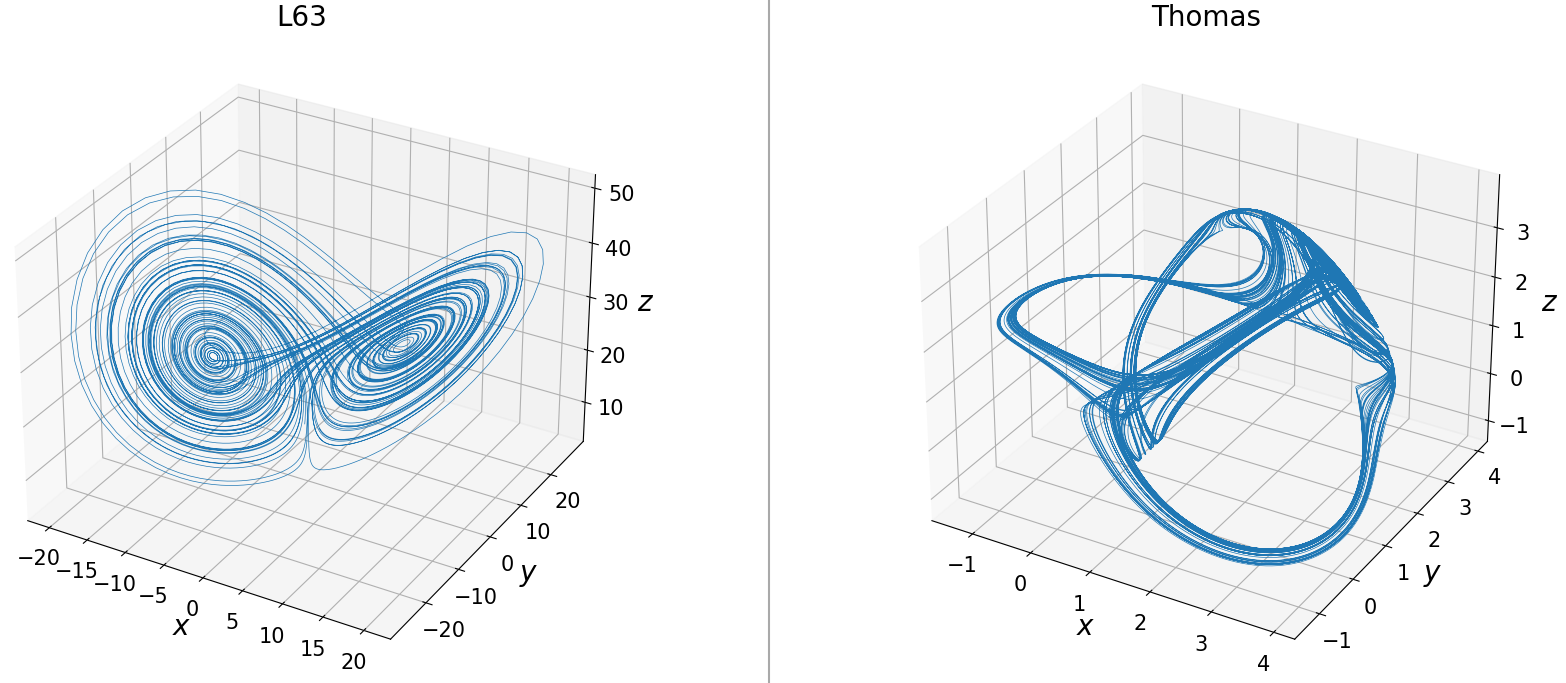
\includegraphics[scale=0.55]{steady-plots/attractor.png}
   \caption{Attractors for non-gradient examples} \label{fig:attractors}
\end{figure}

